\documentclass[9pt]{beamer}

\usetheme[progressbar=frametitle]{metropolis}
\usepackage{appendixnumberbeamer}

\usepackage{booktabs}
\usepackage[scale=2]{ccicons}

\usepackage{pgfplots}
\usepgfplotslibrary{dateplot}
\usepackage{minted}

\usepackage{pdfpages}
\newcommand{\bnabla}{\mbox{\boldmath$\nabla$}}

\usepackage{xspace}
\newcommand{\themename}{\textbf{\textsc{metropolis}}\xspace}


\usepackage[francais]{babel}
\usepackage{amsmath}
\usepackage{amssymb}
\usepackage{amsfonts}
\usepackage{amsthm}

\title{Simulation numérique de convection}
\subtitle{avec le logiciel ASPECT}
% \date{\today}
\date{2021 -- M1STU Nantes}
\author{Marine Lasbleis}


\AtBeginSection[]
{
  \begin{frame}<beamer>
    \frametitle{}
    \tableofcontents[currentsection, hideothersubsections]
  \end{frame}
}

% \titlegraphic{\hfill\includegraphics[height=1.5cm]{logo.pdf}}

\begin{document}

\maketitle




\begin{frame}{Déroulement de la séance}
    \tableofcontents[hideallsubsections]
\end{frame}

\section{Avant de commencer}


\begin{frame}[fragile]{Téléchargements sur }

Merci de vous connecter sur votre session (Linux!)

\vspace{2em}

    Liste des fichiers à télécharger sur Madoc: 
    \begin{itemize}
        \item Ces slides
        \item Notebook jupyter (Python)
        \item Les fichiers de paramètres (.prm)
    \end{itemize}
    
    Créer un dossier spécifique pour y mettre les documents (et y mettre les documents): 

    \begin{minted}{shell-session}
mkdir ./Documents/M1_int_plan/
    \end{minted}
    
    À récupérer sur l'ordinateur: 
    \begin{minted}{shell-session}
cp  /usr/local/opt/aspect/bin/aspect ./Documents/M1_int_plan/
    \end{minted}


\end{frame}

\subsection{Commandes usuelles dans un terminal}
\begin{frame}[fragile]{Commandes usuelles UNIX (terminal)}
ouvrir un terminal sous Ubuntu: Ctrl+Alt+T
   
\begin{itemize}
    \item \textbf{pwd} -- gives absolute path
    \item \textbf{ls} -- lists files in the folder
    \item \textbf{cd <folder\_name>} -- move to <folder\_name>
    
    try also: \textbf{cd}, \textbf{cd ..} and \textbf{cd \~}
    
    \item \textbf{mkdir \& rmdir} -- make new directory, or remove one.
    \item \textbf{rm} -- remove file (-r to remove also directories)
    \item \textbf{man \& --help} -- to get help about a command
    \item \textbf{cp \& mv} -- to copy or move files (-r for directories)
    \item \textbf{locate} -- to locate a file with his name
\end{itemize}
\end{frame}


\begin{frame}[fragile]{Commandes usuelles UNIX (terminal)}
    Quelques commandes supplémentaires utiles:
    \begin{itemize}
        \item \textbf{grep word files} -- to see if files contain the word \textbf{word}.
        \item Text editors: use the one you are the most familiar with. Default should be easy (example: gedit). Other options are nano, vim, emacs. 
        \item Use the autocomplete function: start typing and use TAB to complete the word.
        \item Ctrl+C to stop a command that is running in the current terminal (Ctrl+z if not working). \textbf{top} to check what is running on your computer. 
        \item \textbf{sudo} allows you to use a command as if you are super-user (requires admin right and the password) Default is not to log as admin!
        \item \textbf{apt-get} will install most programs needed. 
    \end{itemize}
    
\end{frame}

\subsection{Lancement d'une simulation}
\begin{frame}[fragile]{Lancement d'une simulation}
    Avant de commencer le cours, on va lancer une simulation: 
    \begin{itemize}
        \item télécharger le fichier .prm de votre groupe (le mettre dans un dossier dans Documents)
        \item ouvrir un terminal
        \begin{minted}{shell-session}
    cd ./Documents/M1_int_plan/
    ./aspect fichier_XX.prm
    \end{minted}
        \item Laisser tourner en tache de fond (ne touchez plus au terminal)
    \end{itemize}
\end{frame}

\subsection{Notebooks jupyter}

\begin{frame}[fragile]{Notebooks jupyter}
    
    Pour le traitement des données, on va utiliser deux systèmes: 
    
    \begin{itemize}
        \item Paraview (visualisation globale)
        \item Python (via des notebooks) pour les statistiques
    \end{itemize}
    
    Pour ouvrir les notebooks jupyter: 
    \begin{itemize}
        \item ouvrir un terminal, se placer dans le dossier adéquat
        \begin{minted}{shell-session}
    cd ./Documents/M1_int_plan/
    jupyter notebook
    \end{minted}
        \item jupyter notebook
        \item cliquer sur le notebook
        \item pour activer une cellule: Shift+Entrée
    \end{itemize}
    
    Chez vous: installer python avec anaconda https://www.anaconda.com/distribution/ 
    
    Pour installer pandas et pyyaml: 
    
    \begin{minted}{shell-session}
    pip3 install pandas pyyaml
\end{minted}
   
\end{frame}

%==============================================


\section{Prise en main d'ASPECT}




\subsection{Le logiciel ASPECT}
\begin{frame}{ASPECT}

    \textbf{A}dvanced \textbf{S}olver for \textbf{P}roblems in \textbf{E}arth’s \textbf{C}onvec\textbf{T}ion
    
    
    Lien vers le manuel:
    
    https://geodynamics.org/cig/software/aspect/aspect-manual.pdf
    
    Permet de simuler des problèmes de convection dans des set-up géophysiques
    \begin{itemize}
        \item Géométries:
        \begin{itemize}
            \item 2D ou 3D
            \item boite, anneau sphérique, sphère
        \end{itemize}
        \item Physique:
        \begin{itemize}
            \item convection simple (approximation de Boussinesq)
            \item compressibilité
            \item fusion et/ou cristallization
            \item convection bi-phasique
            \item topographie
        \end{itemize}
    \end{itemize}
    
    
\end{frame}

{
\setbeamercolor{background canvas}{bg=}
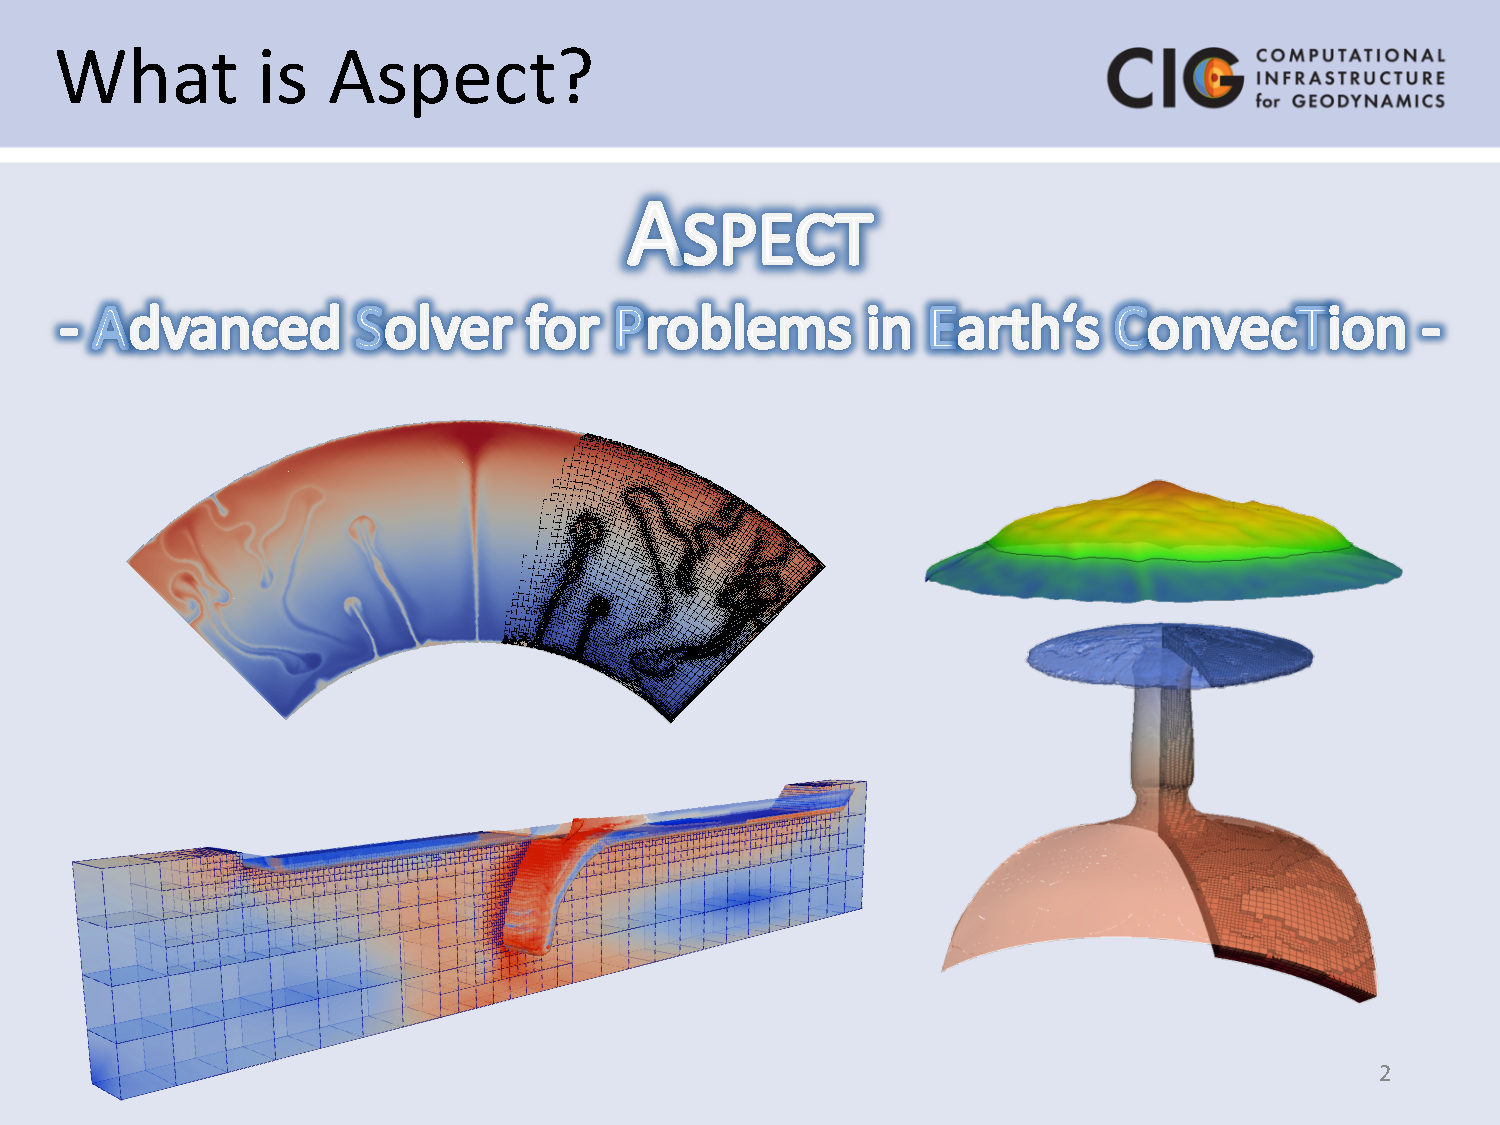
\includepdf[pages=1-3]{aspect_base.pdf}
}



\subsection{Installation}
\begin{frame}{Installation d'ASPECT}
    Lien vers le manuel:
    
    https://geodynamics.org/cig/software/aspect/aspect-manual.pdf
\end{frame}

\subsection{Lancer une simulation}
\begin{frame}[fragile]{Lancer une simulation}
    En se plaçant dans le dossier avec le fichier \textbf{fichier-parametres}.prm:
    \vspace{2em}
    
    
    Avec un seul coeur: 
    \begin{minted}{shell-session}
./aspect fichier-parameters.prm
\end{minted}

    
    Avec plusieurs coeurs (utile si grille fine)
    \begin{minted}{shell-session}
mpirun -np 2 ./aspect fichier-parameters.prm    
\end{minted}

    
\end{frame}
%==============================================

\section{Description du modèle}

\subsection{Modèle physique}
\begin{frame}{Description du modèle}
\begin{minipage}{0.5\textwidth}
\begin{center}
        \includegraphics<2>[width=\linewidth]{drawing.pdf}
\end{center}
\end{minipage}
\hfill
\begin{minipage}{0.49\textwidth}
\begin{itemize}
    \item \textbf{Géométrie} 
    
    boite 2D (infinie en z)
    \item \textbf{Propriétés physiques} 
    
    matériel simple 
    (tout constant, sauf densité qui varie avec les variations de température)
    \item \textbf{Conditions aux limites} 
    
    variation de température entre haut et bas
    
    free-slip partout.
    \item \textbf{Forces extérieures}
    
    gravité constante, orientée vers le bas
\end{itemize}
\end{minipage}
\end{frame}



\subsection{Équations de la dynamique}

\begin{frame}{Équations de la dynamique}
    \textbf{Mots clefs:} équations de conservation (de la quantité de matière, du moment, de l'énergie); pas d'inertie; rhéologie newtonienne à viscosité constante; incompressible; approximation de Boussinesq; Température potentielle $\Theta$; vitesse $\mathbf{v}$;
    
    \textbf{En dimensionné:}
    \begin{equation*}
        \bnabla \cdot \mathbf{v} = 0,
    \end{equation*}
    \begin{equation*}
        -\rho_0 \alpha \Theta g \mathbf{e}_z - \bnabla P +\eta \nabla ^2 \mathbf{v} =\mathbf{0}, 
    \end{equation*}
    \begin{equation*}
        \frac{\partial \Theta}{\partial t}+\mathbf{v}\cdot \bnabla \Theta = \kappa \nabla ^2 \Theta \ \ \ (+ H)
    \end{equation*}
    
    \textbf{En adimensionné:}
    \begin{equation*}
        \bnabla \cdot \mathbf{v} = 0,       
    \end{equation*}
    \begin{equation*}
        Ra \Theta - \bnabla P + \nabla ^2 \mathbf{v} =\mathbf{0}, 
    \end{equation*}
    \begin{equation*}
        \frac{\partial T}{\partial t}+\mathbf{v}\cdot \bnabla T =  \nabla ^2 T \ \ \ (+ H)
    \end{equation*}
\end{frame}

\begin{frame}{Résolution des équations via ASPECT}

    
ASPECT résoud numériquement les équations dans un volume donné en utilisant des méthodes d'élements finis. On discrétise l'espace et le temps. Cela implique de définir une grille (un mesh). ASPECT permet de redéfinir la grille au cours du temps (\textbf{mesh refinement}), ce qui permet dans certains cas d'optimiser le temps de calcul.

    ASPECT utilise les \textbf{grandeurs dimensionnées} en input, mais le type de dynamique dont on s'occupe ici est controlé par un seul nombre sans dimension: le nombre de Rayleigh. 
    
    En faisant varier la gravité, on fait varier le nombre de Rayleigh (et uniquement ce nombre là). 
    
    On peut donc regarder les résultats et voir les différences en fonction du nombre Rayleigh. 
\end{frame}


\subsection{Fichier de paramètres}
\begin{frame}{Fichier de paramètres}
   voir \textbf{fichier}.prm
   
\end{frame}


\subsection{Fichiers de sortie}
\begin{frame}{Fichiers de sortie}
Dans le dossier \textbf{output}: 
\begin{itemize}
    \item \textbf{log.txt} 
    
    toutes les sorties (qui défilent sur le terminal)
    \item \textbf{Fichiers parametres}
    
    parameters.prm (pour réutiliser)
    
    parameters.tex (pour avoir un pdf avec pdflatex)
    \item \textbf{statistics}
    
    Fichier avec 1 ligne par pas de temps résolu, avec les statistiques globales de la simulation.
    \item \textbf{Fichiers de visualisation}
    
    solution.pvd / solution.visit: contient toutes les infos pour ouvrir d'un coup tous les fichiers de sortie.
    
    dossier solution: contient tous les fichiers de sortie.
\end{itemize}
\end{frame}


%==============================================


\section{Description de la dynamique}

\subsection{Visualisation avec Paraview}


\begin{frame}{Visualisation avec Paraview}
 
 \begin{itemize}
    \item Ouvrir le logiciel paraview
    \item File > Open > sélectionner le fichier solution.pvd
    \item Cliquer sur "Apply"
    \item Choisir le champs à visualiser
\end{itemize}
    
\end{frame}


\subsection{Absence de convection}
\begin{frame}{Absence de convection}

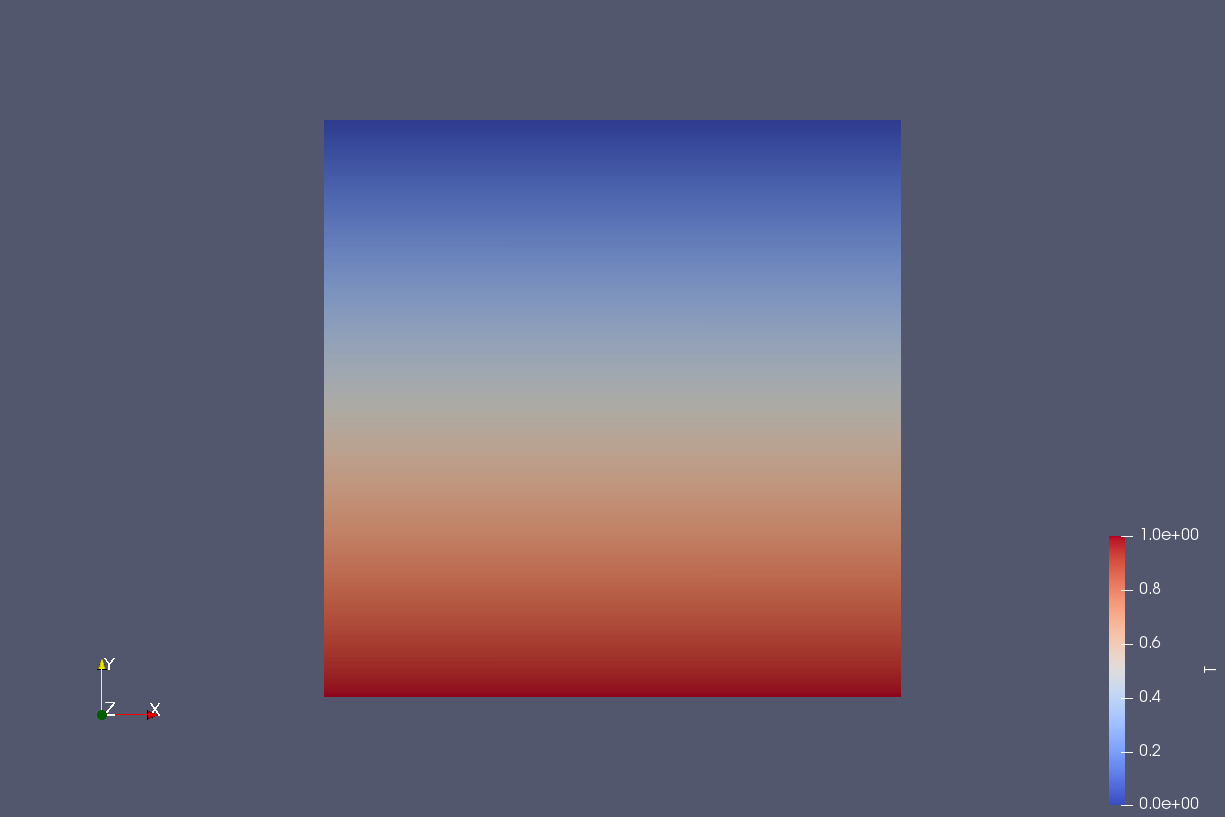
\includegraphics[width=\textwidth]{fig/screen_Ra1e2.png}

    \textbf{Attention}: la vitesse est nulle, le pas de temps est infini (ou presque)...
\end{frame}

\subsection{Bas nombre de Rayleigh}
\begin{frame}{Bas nombre de Rayleigh}
    \includegraphics<1>[width=\textwidth]{fig/screen_Ra1e4.png}
    \includegraphics<2>[width=\textwidth]{fig/screen_Ra1e4_edges.png}
\end{frame}

\subsection{Haut nombre de Rayleigh}
\begin{frame}{Haut nombre de Rayleigh}
    \includegraphics<1>[width=\textwidth]{fig/screen_Ra3e6.png}
    \includegraphics<2>[width=\textwidth]{fig/screen_Ra3e6_edges.png}
   
    \textbf{Attention}: la dynamique est à petite échelle, il faut donc faire attention à la grille.
\end{frame}

\section{Lois d'échelles}

\subsection{Extraire les évolutions temporelles}

\begin{frame}{Fichier statistics}
    voir notebook jupyter
    
    \begin{itemize}
        \item ouvrir un terminal
        \item jupyter notebook
    \end{itemize}
\end{frame}

\begin{frame}{Évolutions temporelles -- Ra=$10^4$}
    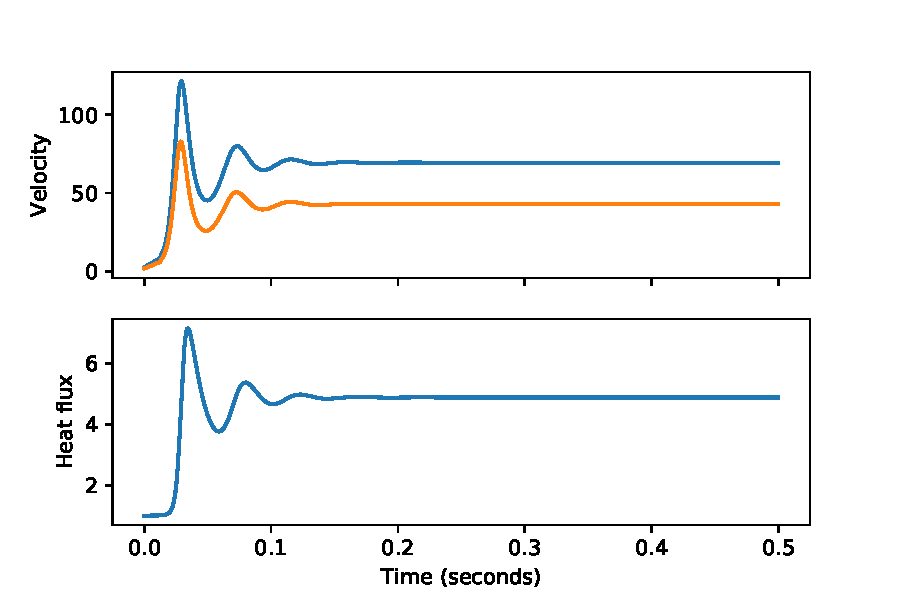
\includegraphics[width=\textwidth]{fig/evolution_temporelle_Ra1e4.pdf}
\end{frame}

\begin{frame}{Évolutions temporelles -- Ra=$3\cdot 10^6$}
    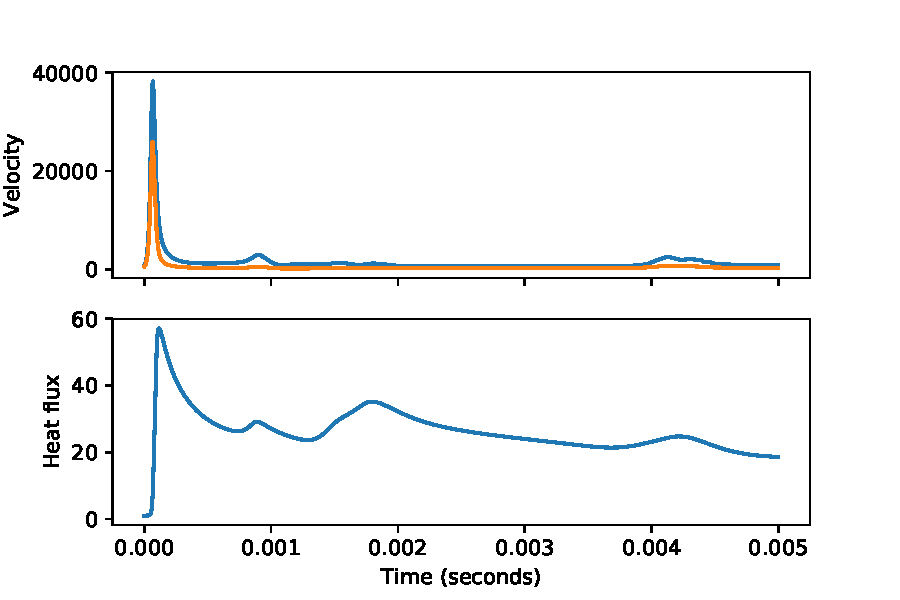
\includegraphics[width=\textwidth]{fig/evolution_temporelle_Ra3e6.pdf}
\end{frame}

\subsection{Lois d'échelles}

\begin{frame}{Lois d'échelles}

Lois Nusselt/Rayleigh: 

Faire une figure avec log(Flux chaleur haut) en fonction de log(Ra)
    
\end{frame}

\section{Profils moyens}

\subsection{Extraire et visualiser les profils moyens}
\begin{frame}{Extraire et visualiser les profils moyens}
    cf notebook Python
\end{frame}

\begin{frame}{Profils moyens -- Ra=$10^4$}
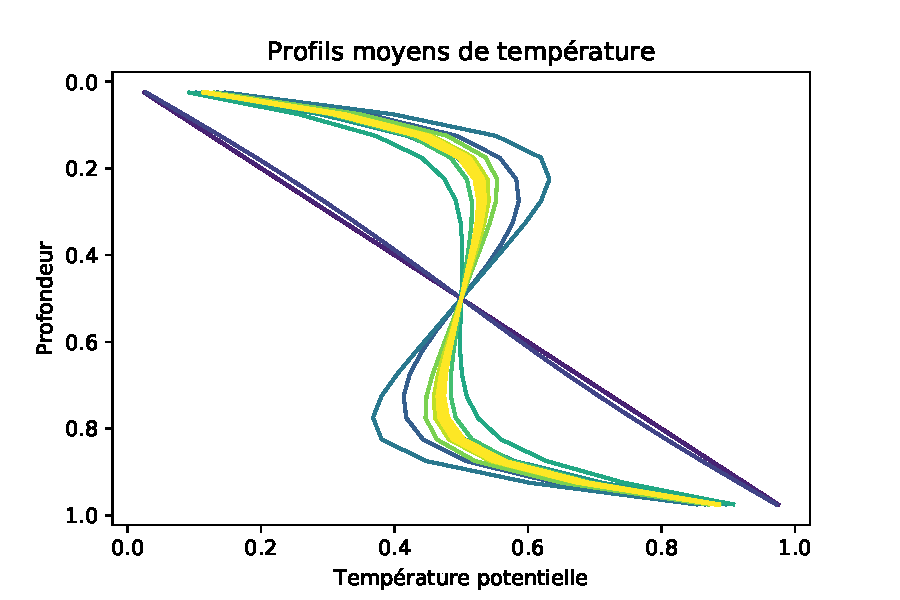
\includegraphics[width=\textwidth]{fig/profils_moyens_Ra1e4.pdf}
\end{frame}

\begin{frame}{Profils moyens -- Ra=$3\cdot 10^6$}
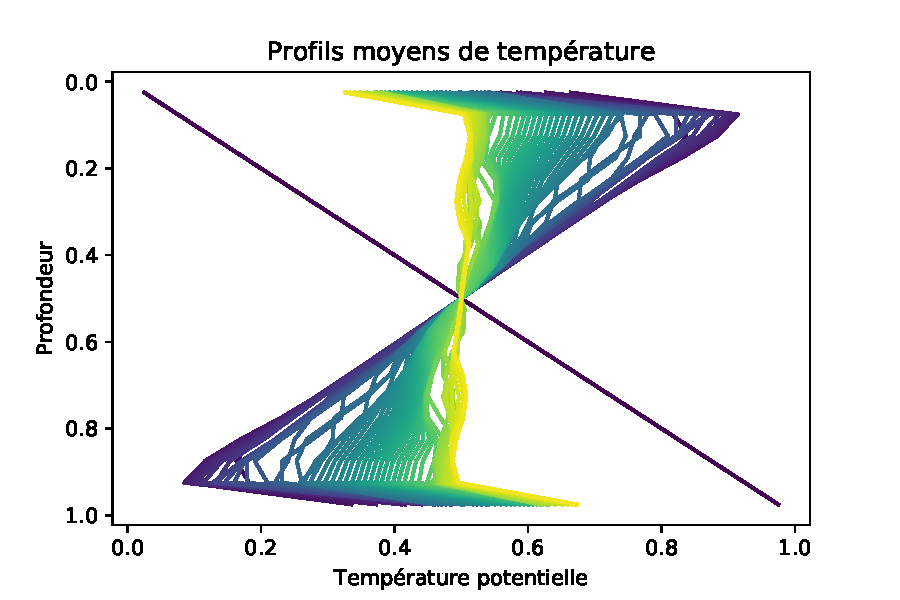
\includegraphics[width=\textwidth]{fig/profils_moyens_Ra3e6.pdf}
\end{frame}

\section{Projets}

\subsection{Structure d'un projet}

\begin{frame}{Structure d'un projet}
    \begin{itemize}
        \item Description physique et numérique du problème
        \item Description des dynamiques obtenues
        \begin{itemize}
            \item Décrire les différents types de dynamique obtenus (en mettant des exemples)
            \item Regarder la convergence pour chacun des cas et montrer un exemple convergé/non convergé.
            \item Étudier les couches limites à partir des profils moyens
            \item possibilité de faire des vidéos avec paraview (mettre en ligne et lien dans projet)
            \item attention sur l'effet du maillage (plus ou moins fin) pour la convergence
        \end{itemize}
        \item Lois Nu-Ra en fonction des paramètres
        \begin{itemize}
            \item tracer le flux de chaleur en surface en fonction du Rayleigh
            \item Remplir le document partagé: 
            https://uncloud.univ-nantes.fr/index.php/s/5xZdFaqBg6wE8KT
        \end{itemize}
        %\item Profils moyens
        %\begin{itemize}
        %    \item regarder les couches limites %(augmenter le nombre dans \textbf{Number of zones})
        %\end{itemize}
        \item Discussion
    \end{itemize}
    Compter $\sim$ 10 pages avec figures.

\end{frame}

%\subsection{Liste des projets}
%\begin{frame}{Liste des projets possibles}
%    \begin{itemize}
%        \item \textbf{Projet 1:} 3 rapports d'aspect différent (tailles de boites)
%        \item \textbf{Projet 2:} viscosité variable, dépendance en température
%        \item \textbf{Projet 3:} conditions aux limites free-slip / no-slip
%        \item \textbf{Projet 4:} chauffage interne et/ou chauffage par le bas
%        \item \textbf{Projet 5:} géométrie en 1/4 d'anneau
%    \end{itemize}
%\end{frame}




%\begin{frame}{Notes}
%        Pour chacun des projets, je vous propose de faire tourner 2 runs sur une machine avec (jusque) 20 coeurs, avec des conditions: (ce n'est absolument pas obligatoire!)
%    \begin{itemize}
%        \item me fournir exactement les fichiers de paramètres et les commandes à utiliser (me donner la commande mpirun avec le nombre de coeurs demandés). Temps de calcul limité à 8h.
%        \item Vérifier que les outputs ne dépassent pas 500Mo. (je coupe au dessus de 200 fichiers .pvd)
%        \item 3 jours pour que je fasse tourner et vous renvoie les résultats. 
%    \end{itemize}
%\end{frame}

\subsection{Notes sur le temps de calcul}

\begin{frame}{Notes sur le temps de calcul}
    \begin{itemize}
        \item Écrire des fichiers de sortie coute cher en temps de calcul (mais est très utile pour le débuguage!)
        \item Avoir une grille plus fine coute cher en temps de calcul (mais une grille trop large ne permet pas de bien résoudre la physique!)
        \item Utiliser plusieurs coeurs permet de réduire le temps de calcul (à condition que le temps passé à communiquer entre les coeurs ne soit pas trop grand! Ne pas utiliser pour des problèmes trop petits, ou avec trop de mesh refinment)
        
    \end{itemize}
    

\end{frame}


\end{document}





\begin{frame}{Table of contents}
  \setbeamertemplate{section in toc}[sections numbered]
  \tableofcontents[hideallsubsections]
\end{frame}

\section{Introduction}

\begin{frame}[fragile]{Metropolis}

  The \themename theme is a Beamer theme with minimal visual noise
  inspired by the \href{https://github.com/hsrmbeamertheme/hsrmbeamertheme}{\textsc{hsrm} Beamer
  Theme} by Benjamin Weiss.

  Enable the theme by loading

  \begin{verbatim}    \documentclass{beamer}
    \usetheme{metropolis}\end{verbatim}

  Note, that you have to have Mozilla's \emph{Fira Sans} font and XeTeX
  installed to enjoy this wonderful typography.
\end{frame}
\begin{frame}[fragile]{Sections}
  Sections group slides of the same topic

  \begin{verbatim}    \section{Elements}\end{verbatim}

  for which \themename provides a nice progress indicator \ldots
\end{frame}

\section{Titleformats}

\begin{frame}{Metropolis titleformats}
	\themename supports 4 different titleformats:
	\begin{itemize}
		\item Regular
		\item \textsc{Smallcaps}
		\item \textsc{allsmallcaps}
		\item ALLCAPS
	\end{itemize}
	They can either be set at once for every title type or individually.
\end{frame}

{
    \metroset{titleformat frame=smallcaps}
\begin{frame}{Small caps}
	This frame uses the \texttt{smallcaps} titleformat.

	\begin{alertblock}{Potential Problems}
		Be aware, that not every font supports small caps. If for example you typeset your presentation with pdfTeX and the Computer Modern Sans Serif font, every text in smallcaps will be typeset with the Computer Modern Serif font instead.
	\end{alertblock}
\end{frame}
}

{
\metroset{titleformat frame=allsmallcaps}
\begin{frame}{All small caps}
	This frame uses the \texttt{allsmallcaps} titleformat.

	\begin{alertblock}{Potential problems}
		As this titleformat also uses smallcaps you face the same problems as with the \texttt{smallcaps} titleformat. Additionally this format can cause some other problems. Please refer to the documentation if you consider using it.

		As a rule of thumb: Just use it for plaintext-only titles.
	\end{alertblock}
\end{frame}
}

{
\metroset{titleformat frame=allcaps}
\begin{frame}{All caps}
	This frame uses the \texttt{allcaps} titleformat.

	\begin{alertblock}{Potential Problems}
		This titleformat is not as problematic as the \texttt{allsmallcaps} format, but basically suffers from the same deficiencies. So please have a look at the documentation if you want to use it.
	\end{alertblock}
\end{frame}
}

\section{Elements}

\begin{frame}[fragile]{Typography}
      \begin{verbatim}The theme provides sensible defaults to
\emph{emphasize} text, \alert{accent} parts
or show \textbf{bold} results.\end{verbatim}

  \begin{center}becomes\end{center}

  The theme provides sensible defaults to \emph{emphasize} text,
  \alert{accent} parts or show \textbf{bold} results.
\end{frame}

\begin{frame}{Font feature test}
  \begin{itemize}
    \item Regular
    \item \textit{Italic}
    \item \textsc{SmallCaps}
    \item \textbf{Bold}
    \item \textbf{\textit{Bold Italic}}
    \item \textbf{\textsc{Bold SmallCaps}}
    \item \texttt{Monospace}
    \item \texttt{\textit{Monospace Italic}}
    \item \texttt{\textbf{Monospace Bold}}
    \item \texttt{\textbf{\textit{Monospace Bold Italic}}}
  \end{itemize}
\end{frame}

\begin{frame}{Lists}
  \begin{columns}[T,onlytextwidth]
    \column{0.33\textwidth}
      Items
      \begin{itemize}
        \item Milk \item Eggs \item Potatos
      \end{itemize}

    \column{0.33\textwidth}
      Enumerations
      \begin{enumerate}
        \item First, \item Second and \item Last.
      \end{enumerate}

    \column{0.33\textwidth}
      Descriptions
      \begin{description}
        \item[PowerPoint] Meeh. \item[Beamer] Yeeeha.
      \end{description}
  \end{columns}
\end{frame}
\begin{frame}{Animation}
  \begin{itemize}[<+- | alert@+>]
    \item \alert<4>{This is\only<4>{ really} important}
    \item Now this
    \item And now this
  \end{itemize}
\end{frame}
\begin{frame}{Figures}
  \begin{figure}
    \newcounter{density}
    \setcounter{density}{20}
    \begin{tikzpicture}
      \def\couleur{alerted text.fg}
      \path[coordinate] (0,0)  coordinate(A)
                  ++( 90:5cm) coordinate(B)
                  ++(0:5cm) coordinate(C)
                  ++(-90:5cm) coordinate(D);
      \draw[fill=\couleur!\thedensity] (A) -- (B) -- (C) --(D) -- cycle;
      \foreach \x in {1,...,40}{%
          \pgfmathsetcounter{density}{\thedensity+20}
          \setcounter{density}{\thedensity}
          \path[coordinate] coordinate(X) at (A){};
          \path[coordinate] (A) -- (B) coordinate[pos=.10](A)
                              -- (C) coordinate[pos=.10](B)
                              -- (D) coordinate[pos=.10](C)
                              -- (X) coordinate[pos=.10](D);
          \draw[fill=\couleur!\thedensity] (A)--(B)--(C)-- (D) -- cycle;
      }
    \end{tikzpicture}
    \caption{Rotated square from
    \href{http://www.texample.net/tikz/examples/rotated-polygons/}{texample.net}.}
  \end{figure}
\end{frame}
\begin{frame}{Tables}
  \begin{table}
    \caption{Largest cities in the world (source: Wikipedia)}
    \begin{tabular}{lr}
      \toprule
      City & Population\\
      \midrule
      Mexico City & 20,116,842\\
      Shanghai & 19,210,000\\
      Peking & 15,796,450\\
      Istanbul & 14,160,467\\
      \bottomrule
    \end{tabular}
  \end{table}
\end{frame}
\begin{frame}{Blocks}
  Three different block environments are pre-defined and may be styled with an
  optional background color.

  \begin{columns}[T,onlytextwidth]
    \column{0.5\textwidth}
      \begin{block}{Default}
        Block content.
      \end{block}

      \begin{alertblock}{Alert}
        Block content.
      \end{alertblock}

      \begin{exampleblock}{Example}
        Block content.
      \end{exampleblock}

    \column{0.5\textwidth}

      \metroset{block=fill}

      \begin{block}{Default}
        Block content.
      \end{block}

      \begin{alertblock}{Alert}
        Block content.
      \end{alertblock}

      \begin{exampleblock}{Example}
        Block content.
      \end{exampleblock}

  \end{columns}
\end{frame}
\begin{frame}{Math}
  \begin{equation*}
    e = \lim_{n\to \infty} \left(1 + \frac{1}{n}\right)^n
  \end{equation*}
\end{frame}
\begin{frame}{Line plots}
  \begin{figure}
    \begin{tikzpicture}
      \begin{axis}[
        mlineplot,
        width=0.9\textwidth,
        height=6cm,
      ]

        \addplot {sin(deg(x))};
        \addplot+[samples=100] {sin(deg(2*x))};

      \end{axis}
    \end{tikzpicture}
  \end{figure}
\end{frame}
\begin{frame}{Bar charts}
  \begin{figure}
    \begin{tikzpicture}
      \begin{axis}[
        mbarplot,
        xlabel={Foo},
        ylabel={Bar},
        width=0.9\textwidth,
        height=6cm,
      ]

      \addplot plot coordinates {(1, 20) (2, 25) (3, 22.4) (4, 12.4)};
      \addplot plot coordinates {(1, 18) (2, 24) (3, 23.5) (4, 13.2)};
      \addplot plot coordinates {(1, 10) (2, 19) (3, 25) (4, 15.2)};

      \legend{lorem, ipsum, dolor}

      \end{axis}
    \end{tikzpicture}
  \end{figure}
\end{frame}
\begin{frame}{Quotes}
  \begin{quote}
    Veni, Vidi, Vici
  \end{quote}
\end{frame}

{%
\setbeamertemplate{frame footer}{My custom footer}
\begin{frame}[fragile]{Frame footer}
    \themename defines a custom beamer template to add a text to the footer. It can be set via
    \begin{verbatim}\setbeamertemplate{frame footer}{My custom footer}\end{verbatim}
\end{frame}
}

\begin{frame}{References}
  Some references to showcase [allowframebreaks] \cite{knuth92,ConcreteMath,Simpson,Er01,greenwade93}
\end{frame}

\section{Conclusion}

\begin{frame}{Summary}

  Get the source of this theme and the demo presentation from

  \begin{center}\url{github.com/matze/mtheme}\end{center}

  The theme \emph{itself} is licensed under a
  \href{http://creativecommons.org/licenses/by-sa/4.0/}{Creative Commons
  Attribution-ShareAlike 4.0 International License}.

  \begin{center}\ccbysa\end{center}

\end{frame}

{\setbeamercolor{palette primary}{fg=black, bg=yellow}
\begin{frame}[standout]
  Questions?
\end{frame}
}

\appendix

\begin{frame}[fragile]{Backup slides}
  Sometimes, it is useful to add slides at the end of your presentation to
  refer to during audience questions.

  The best way to do this is to include the \verb|appendixnumberbeamer|
  package in your preamble and call \verb|\appendix| before your backup slides.

  \themename will automatically turn off slide numbering and progress bars for
  slides in the appendix.
\end{frame}

\begin{frame}[allowframebreaks]{References}

  \bibliography{demo}
  \bibliographystyle{abbrv}

\end{frame}

\end{document}
